\documentclass[a4paper,10pt]{article}
\usepackage[utf8]{inputenc}
\usepackage{natbib}
\usepackage{graphicx}
\usepackage{alltt}
\usepackage{latexsym}
\usepackage{vmargin}
\usepackage{wrapfig}
\usepackage{amsmath,amsfonts,amssymb,amscd,amsthm,xspace}

%----------------------------------------------------------------------------------------
%	MARGINS
%----------------------------------------------------------------------------------------
\setmarginsrb  { 1.5in}  % left margin
                        { 0.6in}  % top margin
                        { 1.0in}  % right margin
                        { 0.8in}  % bottom margin
                        {  20pt}  % head height
                        {0.25in}  % head sep
                        {   9pt}  % foot height
                        { 0.3in}  % foot sep
%----------------------------------------------------------------------------------------

%----------------------------------------------------------------------------------------
%	Superscript and subscript code
%----------------------------------------------------------------------------------------
 
\makeatletter
\newcommand\textsubscript[1]{\@textsubscript{\selectfont#1}}
\def\@textsubscript#1{{\m@th\ensuremath{_{\mbox{\fontsize\sf@size\z@#1}}}}}
\newcommand\textbothscript[2]{%
  \@textbothscript{\selectfont#1}{\selectfont#2}}
\def\@textbothscript#1#2{%
  {\m@th\ensuremath{%
    ^{\mbox{\fontsize\sf@size\z@#1}}%
    _{\mbox{\fontsize\sf@size\z@#2}}}}}
\def\@super{^}\def\@sub{_}
\catcode`^\active\catcode`_\active
\def\@super@sub#1_#2{\textbothscript{#1}{#2}}
\def\@sub@super#1^#2{\textbothscript{#2}{#1}}
\def\@@super#1{\@ifnextchar_{\@super@sub{#1}}{\textsuperscript{#1}}}
\def\@@sub#1{\@ifnextchar^{\@sub@super{#1}}{\textsubscript{#1}}}
\def^{\let\@next\relax\ifmmode\@super\else\let\@next\@@super\fi\@next}
\def_{\let\@next\relax\ifmmode\@sub\else\let\@next\@@sub\fi\@next}
\makeatother


%opening
\title{Topic models for Sentiment analysis: \\ A Literature Survey}
\author{Nikhilkumar Jadhav \\
	123050033}

\begin{document}

\maketitle

% \begin{abstract}
% 
% \end{abstract}
In this report, we present the work done so far in the field of sentiment analysis
using topic models. The roadmap of the report is as follows. In section~\ref{sec1},
we introduce topic models. Section~\ref{sec2} discusses the applications of
topic models. Finally, in section~\ref{sec3} we explain how some works have made
use of topic models for sentiment analysis.


\section{Introduction to Topic models}\label{sec1}

\indent Bayesian networks are a formal graphical language to express the joint distribution of 
a system or phenomenon in terms of random variables and their conditional dependencies
in a directed graph \citep*{heinrich2005parameter}. A generative model is a bayesian 
network which provides an intuitive description of an observed phenomenon which states
how observations could have been generated by realizations of random variables and 
their propagation along the directed edges of the network \citep*{heinrich2005parameter}.
Topic models are probabilistic generative models. Topic models try to model the text 
and usually the generation process of text by means of a bayesian network. \\


\textit{Latent Dirichlet Allocation} (\textit{LDA}) is one of the most popular topic models \citep*{blei2003latent}.
Here, the word \emph{latent} signifies capturing the meaning of the text by finding out the 
hidden topics. It identifies the topic structure in text using co-occurrence structure of
terms. It is completely unsupervised as it does not require any background knowledge. The
model is as show in figure \ref{lda}. The replication of a node is represented by a \textit{plate}. 
This is to account for multiple values or mixture components. Let us have a look at the
generative process of \textit{LDA}.

% \begin{wrapfigure}{r}{0.5\textwidth}
%   \vspace{-10pt}
%   \begin{center}
%     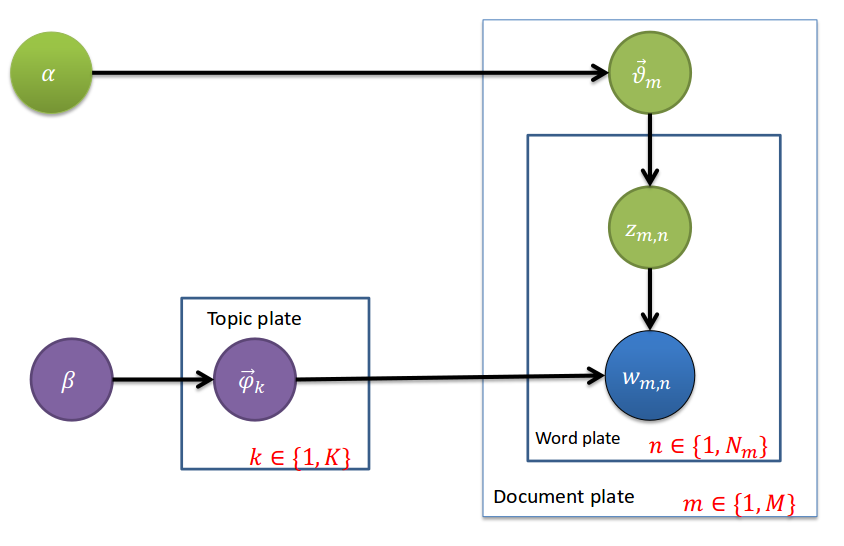
\includegraphics[width=0.45\textwidth]{lda}
%   \end{center}
%   \vspace{-10pt}
%   \caption{LDA}
%   \vspace{-10pt}
% \end{wrapfigure}

\begin{figure}[h!]
   \centering
     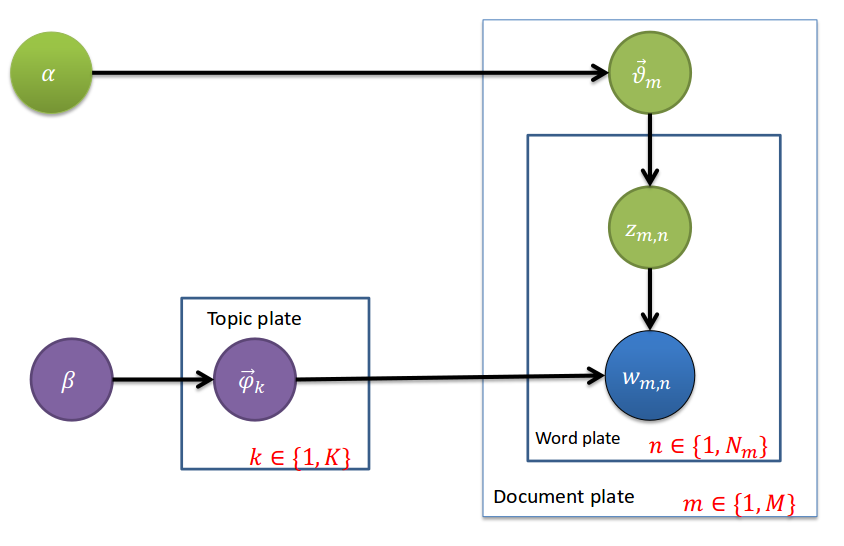
\includegraphics[width=0.7\textwidth]{lda}
   \caption{Latent Dirichlet Allocation}
   \label{lda}
\end{figure}

\subsection{Generative Model for LDA}

Let us describe the quantities used in the model

\begin{alltt}
\(M\) number of documents to generate (const scalar).
\(K\) number of topics/mixture components (const scalar).
\(V\) number of terms \(t\) in vocabulary (const scalar).
\(\vec{\alpha}\) hyper-parameter on the mixing proportions (\(K-vector\) or scalar if symmetric).
\(\vec{\beta}\) hyper-parameter on the mixing components (\(K-vector\) or scalar if symmetric).
\(\vec{\vartheta}_m\) parameter notation for p(z|d=m), the topic mixture proportion for document \(m\). 
  One proportion for each document, \(\underline{\theta} = \{\vec{\vartheta}_m\} m=1 \cdots M (M \times K matrix)\).
\(\vec{\psi}_k\) parameter notation for p(t|z=k), the mixture component of topic \(k\). 
  One component for each topic, \(\underline{\phi} = \{\vec{\psi}_k\} k=1 \cdots K (K \times V matrix)\).
\(N_m\) document length (document-specific), here modeled with a Poisson distribution with 
  constant parameter \(xi\).
\(z_{m,n}\) mixture indicator that chooses the topic for the nth word in document m.
\(w_{m,n}\) term indicator for the nth word in document m.
\end{alltt}

\subsection{Generative Process for LDA}

The generative process for \textit{LDA} is as follows\(\colon\)

\begin{alltt}
\(\Box\) Topic Plate \(\colon\)
\textbf{for} all topics \( k \in [1,K] \) \textbf{do}
  sample mixture components \( \vec{\psi_k} \sim Dir(\vec{\beta}) \)
\textbf{end for}
\(\Box\) Document Plate \(\colon\)
\textbf{for} all documents \( m \in [1,M] \) \textbf{do}
  sample mixture proportion \( \vec{\vartheta_m} \sim Dir(\vec{\alpha}) \)
  sample document length \( N_m \sim Poiss(\xi)\)
  \(\Box\) Word Plate \(\colon\)
  \textbf{for} all words \( n \in [1,N_m] \) in document m \textbf{do}
    sample topic index \( z_{m,n} \sim Mult(\vec{\vartheta}_m) \)
    sample term for word \( w_{m,n} \sim Mult(\vec{\psi}_{z_{m,n}}) \)
  \textbf{end for}
\textbf{end for}
\end{alltt}

\subsection{Generative Process in Simple Terms}

\begin{itemize}

\item When writing each document, you decide on the number of words N the document will have.

\item Choose a topic mixture for the document using dirichlet hypergenerator.

\item Generate each word in the document by:
  
  \begin{enumerate}
  
  \item First pick a topic using the multinomial distribution generated from the dirichlet hypergenerator.
  
  \item Then using the topic and the word-topic distribution to generate the word itself.

  \end{enumerate}

\end{itemize}

Assuming this generative model for a collection of documents, LDA then tries to backtrack from the documents 
to find a set of topics that are likely to have generated the collection.

\subsection{Inference via Gibbs Sampling}

The exact inference is intractable in case of \textit{LDA}. An approximate inference via \textit{Gibbs} sampling is used. 
\textit{Gibbs} Sampling \citep*{walsh2004markov} is a special case of \textit{Markov-chain Monte Carlo}. \textit{MCMC} can 
emulate high dimensional probability distributions, \(p(\vec{x})\) by the stationary distribution of a \textit{Markov chain}. 
Each sample is generated for each transition in the chain. This is done after a stationary state of the chain has been reached 
which happens after a so-called ``burn-in period'' which eliminates the effect of initialization parameters. In \textit{Gibbs} 
sampling, the dimensions \(x_i\) of the distribution are sampled alternately one at a time, conditioned on the values of all 
other dimensions, denoted by \(\vec{x}_{ \neg i}\). The full conditional obtained after inference is as given below,

\begin{align}
p(z_i=k|\vec{z}_{\neg i},\vec{w})	& = \frac{p(\vec{w},\vec{z})}{p(\vec{w},\vec{z}_{\neg i})} \\
					& = \frac{p(\vec{w}|\vec{z})p(\vec{z})}{p(\vec{w}|\vec{z}_{\neg i})p(\vec{z}_{\neg i})} \\
					& \propto \frac{\Delta(\vec{n}_z+\vec{\beta})}{\Delta(\vec{\beta})} . \frac{\Delta(\vec{n}_m+\vec{\alpha})}{\Delta(\vec{\alpha})} \\
					& \propto \frac{\Gamma(n_{k}^{(t)} + \beta_t)\Gamma(\sum_{t=1}^{V} n_{k,\neg i}^{(t)} + \beta_t)}{\Gamma(n_{k,\neg i}^{(t)} + \beta_t)\Gamma(\sum_{t=1}^{V} n_{k}^{(t)} + \beta_t)}.
						  \frac{\Gamma(n_{m}^{(k)} + \alpha_k)\Gamma(\sum_{k=1}^{K} n_{m,\neg i}^{(k)} + \beta_t)}{\Gamma(n_{m,\neg i}^{(k)} + \beta_t)\Gamma(\sum_{k=1}^{K} n_{m}^{(k)} + \beta_t)} \\
					& \propto \frac{n_{k,\neg i}^{(t)} + \beta_t}{\sum_{t=1}^{V}n_{k,\neg i}^{(t)} + \beta_t}.
						  \frac{n_{m,\neg i}^{(k)} + \alpha_k}{[\sum_{k=1}^{K}n_{m,\neg i}^{(k)} + \alpha_k]-1}
					\label{eqn:fullconditionalfinal}
\end{align}

\subsubsection*{Multinomial Parameters}

The multinomial parameter sets, \(\underline{\Theta}\) and \(\underline{\phi}\) that correspond to the state of the Markov
chain, \(M={\vec{w},\vec{z}}\) can be obtained as follows

\begin{equation}\label{eqn:multtheta}
p(\vec{\vartheta}_m|M,\vec{\alpha}) = \frac{1}{Z_{\vartheta_m}} \prod_{n=1}^{N_m} p(z_{m,n}|\vec{\vartheta}_m) p(\vec{\vartheta}_m|\vec{\alpha}) = 	Dir(\vec{\vartheta}_m|\vec{n}_m + \vec{\alpha})
\end{equation}

\begin{equation}\label{eqn:multphi}
p(\vec{\psi}_k|M,\vec{\beta}) = \frac{1}{Z_{\psi_k}} \prod_{k=1}^{K} p(w_{i}|\vec{\psi}_k) p(\vec{\psi}_k|\vec{\beta}) = 	Dir(\vec{\psi}_k|\vec{n}_k + \vec{\beta}) 
\end{equation}

Using the expectation of the dirichlet distribution, \(Dir(\vec{\alpha}) = \frac{a_i}{\sum_i a_i}\) in equation \ref{eqn:multtheta} and equation \ref{eqn:multphi} we get,

\begin{equation}\label{eqn:phi}
\psi_{k,t} = \frac{n_k^{(t)} + \beta_t}{\sum_{t=1}^{V} n_k^{(t)} + \beta_t}
\end{equation}

\begin{equation}\label{eqn:theta}
\vartheta_{m,k} = \frac{n_m^{(k)} + \alpha_t}{\sum_{k=1}^{K} n_m^{(k)} + \alpha_k} 
\end{equation}

\subsection{Gibbs Sampling Algorithm for LDA}

\begin{alltt}
\(\Box\) Initialization
zero all count variables, \(n_m^{(k)},n_m,n_k^{(t)},n_k\)
for all documents \(m \in [1,M]\) do
  for all words \(n \in [1,N_m]\) in document \(m\) do
    sample topic index \(z_{m,n} = k \sim Mult(1/K)\)
    increment document-topic count: \(n_m^{(k)} + 1\)
    increment document-topic sum: \(n_m + 1\)
    increment topic-term count: \(n_k^{(t)} + 1\)
    increment topic-term sum: \(n_k + 1\)
  end for
end for
\(\Box\) Gibbs sampling over burn-in period and sampling period
while not finished do
  for all documents \(m \in [1,M]\) do
    for all words \(n \in [1,N_m]\) in document \(m\) do
      \(\Box\) for the current assignment of \(k\) to a term \(t\) for word \(w_{m,n}\) \(\colon\)
      decrement counts and sum:\(n_m^{k}-1,n_m-1,n_k^{(t)}-1,n_k-1\)
      \(\Box\) multinomial sampling according to equation \ref{eqn:fullconditionalfinal} (decrements from the previous step)
      sample topic index \(\bar{k} \sim p(z_i|\vec{z}_{\neg i},\vec{w})\)
      \(\Box\) use the new assignment of \(z_{m,n}\) to the term \(t\) for word \(w_{m,n}\) to:
      increment the counts and sum:\(n_m^{k}+1,n_m+1,n_k^{(t)}+1,n_k+1\)
    end for
  end for
  \(\Box\) check convergence and read out parameters
  if converged ad \(L\) sampling iterations since last read out then
    \(\Box\) the different parameters read outs are averaged
    read out parameter set \(\underline{\phi}\) according to equation \ref{eqn:phi}
    read out parameter set \(\underline{\theta}\) according to equation \ref{eqn:theta}
  end if
end while
\end{alltt}

\subsection{Gibbs Sampling Algorithm in Simple Terms}

We should note one important fact that our hidden variable is \(z\) i.e., the topic assignment to each word.

\begin{itemize} 
 \item Go through each document and randomly assign each word in the document one of the \(K\) topics.
 \item This random assignment gives you both \textbf{topic-document} distribution and \textbf{word-topic} 
 distributions but not very good ones.
 \item To improve them, we compute two things, \(p(t|d)\) and \(p(w|t)\).
 \item After that, reassign each word \(w\) a new topic, where the topic t is chosen with probability
 \(p(t|d) \times p(w|t)\)
 \item We assume that all the topic assignments except for the current word is question are correct,
 and then update the assignment of the current word using the model. After a suitable number of iteration,
 we get proper topic-document and word-topic distributions.
\end{itemize}

The trained model can then be used to perform inferencing as described next.

\subsection{Inferencing for New Documents}

Inferencing is the process of finding out the topic distribution in a new document. Suppose the new document is represented by \(\bar{m}\),
Let us represent a new document by \(\vec{w}\). We need to find out the posterior distribution of topics \(\vec{z}\) given the word 
vector of the document \(\vec{w}\) and the \textit{LDA Markov} state, \(M = \{ \vec{z},\vec{w} \} \colon p(\vec{z},\vec{w};M) \). The algorithm
is a modification the \textit{Gibbs} sampling algorithm we saw. It starts of by randomly assigning topics to words and then performs number 
of loops through the \textit{Gibbs} sampling update (locally for the words \(i\) of \(\bar{m}\)) \citep*{heinrich2005parameter}.

\begin{equation}\label{eqn:inferencereqn}
p(\bar{z}_i=k | \bar{w}_i=t,\bar{\vec{z}}_{\neg i},\bar{\vec{w}}_{\neg i};M) =
\frac{n_{k}^{(t)} + \bar{n}_{k,\neg i}^{(t)} + \beta_t}{\sum_{t=1}^{V} n_{k}^{(t)} + \bar{n}_{k,\neg i}^{(t)} + \beta_t}.
\frac{n_{\bar{m},\neg i}^{(k)} + \alpha_k}{[\sum_{k=1}^{K} n_{\bar{m},\neg i}^{(k)} + \alpha_k]-1}
\end{equation}

where \(\bar{n}_{k}^{t}\) counts the observations of term \(t\) and topic \(k\) in the new document. \\

The topic distribution of the new document can be found out using the following equation,

\begin{equation}
\vartheta_{\bar{m},k} = \frac{n_{\bar{m}}^{(k)} + \alpha_k}{\sum_{k=1}^{K} n_{\bar{m}}^{(k)} + \alpha_k} 
\end{equation}

Now that we have a basic idea about what topic models are graphically and mathematically, we can discuss some of their applications.

\section{Applications of Topic models}\label{sec2}

\textit{LDA} gives two outputs, \textbf{word-topic} distribution and \textbf{topic-document}. The applications mainly use these two outputs.
First we will focus on the word-topic distribution

\subsection{Applications of Word-Topic Distribution}

\begin{enumerate}
 \item \textit{List of top words in a given topic} \\
 Using the the word-topic distribution, we can get a list of top \(n\) words in any given topic.
 \item \textit{Clustering of Words by topic} \\
 This distribution can also be used to cluster new words based on the co-occurrence principle.
\end{enumerate}


\subsection{Applications of Topic-Document Distribution}

Let us have a look at the applications which use the topic-document distribution.

\begin{enumerate}
 \item \textbf{Similarity Ranking} \\
  We can find the topic distribution for each of the document and compare them for similarity. As these are probability distributions, we make use of a modified
  KL-divergence method to do this.
  
 \item \textbf{Querying} \\
  Querying makes use of similarity ranking to find the documents which are most similar to a given a query.
 
 \item \textbf{Clustering} \\
  Documents can be clustered as per their major topic.
 
 \item \textbf{Document classification} \\
  The topic having highest proportion in the document will be it's class.
 
\end{enumerate}


In the next section, we will look at some attempts to combine topic and sentiment in a generative modeling framework.

\section{Topic models for Sentiment Analysis}\label{sec3}

We will have a look at the following models one by one.

\begin{enumerate}
 \item A Generative model for sentiment \citep*{eguchi2006sentiment}
 \item Topic Sentiment Mixture model \citep*{mei2007topic}
 \item Joint Sentiment Topic model \citep*{lin2009joint}
 \item Aspect-Sentiment Unification model \citep*{jo2011aspect}
\end{enumerate}

\subsection{A Generative model for sentiment}

Sentiment Analysis has been used in Information Retrieval to improve the performance. Information Retrieval was mainly concerned with factual/objective data. So, 
intuitively we see that subjectivity classification can aid information retrieval. \citep*{riloff2005exploiting} has work based on it in which they try to exploit 
subjectivity analysis to improve performance of information extraction. Corpus models are useful in fetching documents specific to a certain topic. Sometimes a user
might need to fetch documents which have a specific sentiment. One such work on sentiment retrieval using generative models is seen in \citep*{eguchi2006sentiment}. 
In this work, they have assumed that user inputs both query terms as well as indicates the desired sentiment polarity in some way. They have combined sentiment and 
topic relevance models to retrieve documents which are most relevant to such user requests. This approach is very important for sentiment aware information retrieval. 
The expression of sentiment in the text is topic dependent. Negative review for a voting event may be expressed using \textit{flawed}. On the other hand negative 
review of politician may be expressed using \textit{reckless}. Sentiment polarity is topic dependent \citep*{engstrom2004topic}. The adjective \textit{unpredictable} 
will have a negative orientation in a car review and it will have a positive orientation in a movie review. 

\subsubsection*{Terminology}

The goal of the model is to generate a collection of sentences \(s_1,s_2,\dots,s_n\). Every document is composed of words \(w_1,w_2,\dots,w_n\) drawn from the vocabulary
\(V\). A binary variable \(b_{ij} \in \{S,T\}\) is used to represent whether a word in position \(j\) in sentence \(i\) is a topic word or a sentiment word. Let \(x_i\)
be the polarity for the sentence \(s_i\). \(x_i\) is a discrete random variable with three outcomes \(\{-1,0,+1\}\). A statement \(s_i\) is represented as a set 
\(\{w_i^s,w_i^t,x_i\}\) where \(w_i^s\) are the sentiment bearing words, \(w_i^t\) are the topic bearing words and \(x_i\) is the sentence polarity. The user query will
be represented in a similar fashion \(\{q_i^s,q_i^t,q^x\}\). Let \(p\) denote a unigram language model. \(P\) denotes the set of all possible language models. It is the
probability simplex. Similarly, let \(p_x\) denote the distribution over three possible polarity values and \(P_x\) will be the corresponding ternary probability simplex.
The function \(\pi:P \times P \times P_x\to[0,1]\) is a function which assigns a probability \(\pi(p_1,p_2,p_x)\) to a pair of language models \(p_1\) and \(p_2\) together
with \(p_x\).

\subsubsection*{Generative model of sentiment}

A sentence \(s_i\) containing words \(w_1,w_2,\dots,w_j,\dots,w_m\) is generated in the following way:

\begin{enumerate}
 \item Draw \textit{p_t, p_s and p_x} from \(\pi (\cdot,\cdot,\cdot)\).
 \item Sample \(x_i\) from a polarity distribution \(p_x(\cdot)\).
 \item For each position \(\textit{j = 1\dots m}\):
  \begin{itemize}
   \item if \(b_{ij}=T\): draw \(w_{j}\) from \(p_t(\cdot)\);
   \item if \(b_{ij}=S\): draw \(w_{j}\) from \(p_s(\cdot)\)
  \end{itemize}
\end{enumerate}

The probability of observing the new statement \(s_i\) containing words \(w_1,w_2,\dots,w_j,\dots,w_m\) is given by:

\begin{equation}
\sum_{p_t,p_s,p_x} \pi(p_t,p_s,p_x)p_x(x_i) \prod_{j=1}^m \left\{ 
  \begin{array}{l l}
    p_t(w_j) & \quad \text{if b_{ij} = T}\\
    p_s(w_j) & \quad \text{otherwise}
  \end{array} \right.
\end{equation}

The probability functions are dirichlet smoothed models and \(\pi(p_1,p_2,p_x)\) is a non-parametric function. 

Each sentence is represented as a bag of words model and the model makes strong independence assumptions. But, due to joint probability distribution used it is able to
model co-occurrence. 

\subsubsection*{Retrieval using the model}

Suppose we are given a collection of statement \(C\) and a query \(\{q_i^s,q_i^t,q^x\}\) given by the user. The topic relevance model \(R_t\) and the sentiment relevance
model \(R_t\) are estimated. For each word \(w\) in a statement within a collection \(C\), these models are estimated as follows:


\begin{equation}
R_t(w) = \frac{P(q^s,q^t\circ w,q^x)}{P(q^s,q^t,q^x)} , R_s(w) = \frac{P(q^s \circ w,q^t,q^x)}{P(q^s,q^t,q^x)} 
\end{equation}

\(q \circ w\) means appending \(w\) to the list \(q\). The statements are ranked using a variation of cross-entropy,

\begin{equation}
 \alpha \sum_v R_t(v) \log p_t (v) + (1-\alpha) \sum_v R_s(v) \log p_s(v)
\end{equation}

\par

The experiments using this approach have shown promising results. This shows that sentiment aware IR can benefit from this technique. As corpus models have been widely 
used in IR, extending and tuning them for SA aware IR can yield good results. 

\subsection{TSM}

\citep*{mei2007topic} proposed the topic sentiment mixture model. Figure \ref{tsm} shows the model. The \textit{TSM} model helps to address the following problems.

\begin{enumerate}
 \item \textbf{Learning General Sentiment models} \\
 Learn a sentiment model for positive opinions and a sentiment model for negative opinions, which are general enough to be used in new unlabeled collections.
 \item \textbf{Extracting Topic models and Sentiment Coverages} \\
 Given a collection of Weblog articles and the general sentiment models learned, customize the sentiment models to this collection, extract the topic models, and 
 extract the sentiment coverages.
 \item \textbf{Modeling Topic Life Cycle and Sentiment Dynamics} \\
 Model the life cycles of each topic and the dynamics of each sentiment associated with that topic in the given collection. 
\end{enumerate}

\begin{figure}[h!]
   \centering
     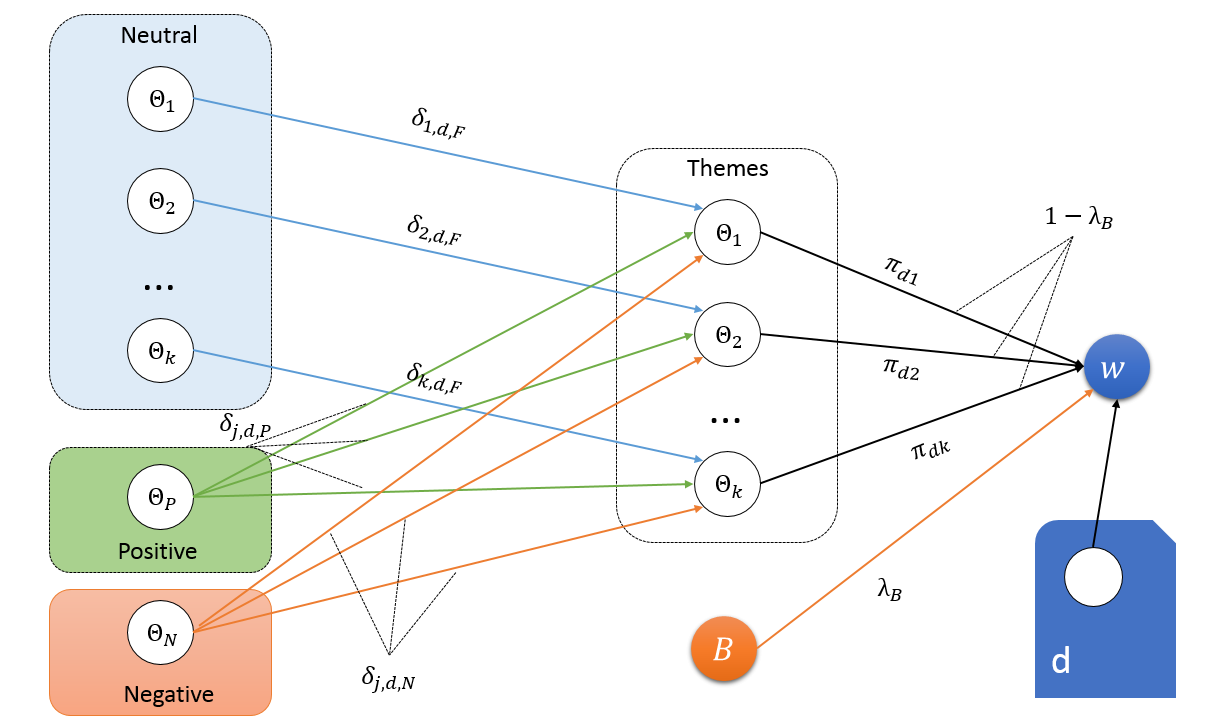
\includegraphics[width=\textwidth]{TSM}
   \caption{Topic Sentiment Mixture Model}
   \label{tsm}
\end{figure}

\subsubsection*{Word Categories}

It divides the words in the document into two major classes
\begin{enumerate}
 \item \textbf{Common English words} e.g., ``the'', ``a'', ``of'', etc.
 \item \textbf{Topic words} eg., ``nano'', ``price'', ``mini'' in the document about \textit{iPod}. The topic words are further divided into three classes.
 \begin{enumerate}
  \item words about the topic with \textbf{neutral} opinion
  \item words about the topic with \textbf{positive} opinion
  \item words about the topic with \textbf{negative} opinion
 \end{enumerate}
\end{enumerate}

\subsubsection*{Multinomials}

There are four multinomial distributions to take note of 
\begin{enumerate}
 \item \(\theta_B\) is a background topic model to capture common English words.
 \item \(\theta = {\theta_1 , ..., \theta_k }\) are \(k\) topic models to capture neutral descriptions about \(k\) global subtopics in the collection.
 \item \(\theta_P\) is a positive sentiment model to capture positive opinions for all the topics in the collection.
 \item \(\theta_N\) is a negative sentiment model to capture negative opinions for all the topics in the collection.
\end{enumerate}

\subsubsection*{Generation Process}

An author follows the procedure given below to generate each word of the document.

\begin{enumerate}
 \item The author would first decide whether the word will be a common English word. If so, the word would be sampled according to \(\theta_B\).
 \item If not, the author would then decide which of the \(k\) subtopics the word should be used to describe. 
 \item Once the author decides which topic the word is about, the author will further decide whether the word is used to describe the topic neutrally, positively,
 or negatively.  
 \item Let the topic picked in step 2 be the \(jth\) topic \(\theta_j\) . The author would finally sample a word using \(\theta_j\), \(\theta_P\) or \(\theta_N\), according 
 to the decision in step 3
\end{enumerate}

The accuracy of the model can be increased by providing domain specific lexicons.

\subsection{Joint Sentiment Topic model}

\citep*{lin2009joint} discusses a joint model of sentiment and topics. Figure \ref{jst} shows the model.


\begin{figure}[h!]
   \centering
     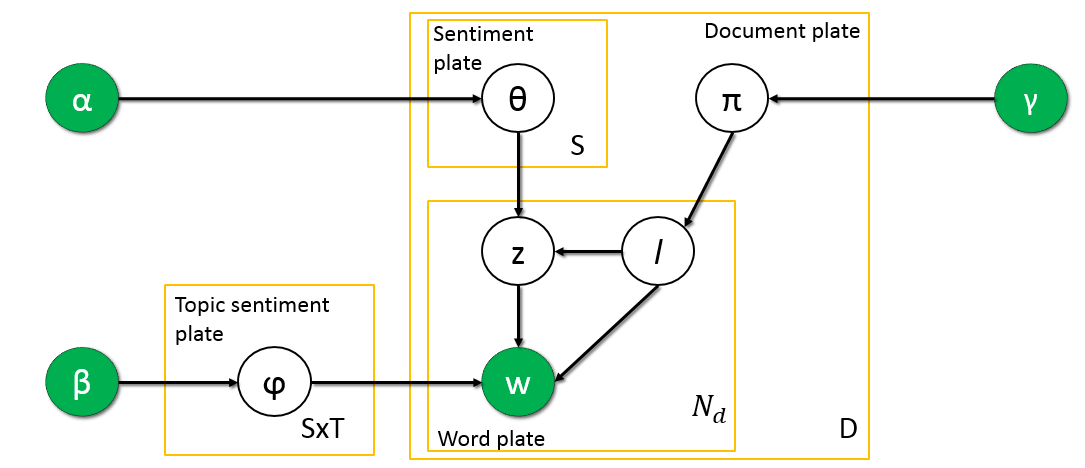
\includegraphics[width=\textwidth]{jst}
   \caption{Joint Sentiment Topic model}
   \label{jst}
\end{figure}

Assume that we have a collection of \(D\) documents denoted by \(C = {d_1,d_2,\cdots,d_D} \); each document in the corpus is a sequence of \(N_d\) words denoted by 
\(d = (w_1,w_2,\cdots,w_{N_d}) \) and each word in the document is an item from a vocabulary index with V distinct terms denoted by \({1,2,\cdots,V}\). Let \(S\) and 
\(T\) be the number of distinct sentiment and topic labels respectively. The procedure of generating a document is described as follows.

\begin{alltt}
For each document \(d\), choose a distribution \(\pi_d \sim Dir(\gamma)\).
For each sentiment label \(l\) under document \(d\), choose a distribution
\(\theta_{d,k} \sim Dir(\alpha)\).
For each word \(w_i\) in document \(d\)
  - choose a sentiment label \(l_i \sim \pi_d\),
  - choose a topic \(z_i \sim \theta_{d,l_i}\),
  - choose a word \(w_i\) from the distribution over words defined by the 
    topic \(z_i\) and sentiment label \(l_i\), \(\psi_{z_i}^{l_i}\)
\end{alltt}


The hyper-parameter \(\alpha\) in \textit{JST} is the prior observation count for the number of times topic \(j\) is associated with  sentiment label \(l\) sampled from
a document. \\

The hyper-parameter \(\beta\) is the prior observation count for the number of times words sampled from topic \(j\) are associated with sentiment label \(l\). \\

Similarly, the hyper-parameter \(\gamma\) is the prior observation count for the number of times sentiment label \(l\) is associated with a document. \\

The latent variables of interest in \textit{JST} are
\begin{enumerate}
 \item The joint sentiment/topic-document distribution, \(\theta\)
 \item The joint sentiment/topic-word distribution, \(\phi\)
 \item The joint sentiment-document distribution, \(\pi\)
\end{enumerate}

To obtain the distributions for \(\theta\), \(\phi\), and \(\pi\), we firstly estimate the posterior distribution over \(z\) i.e, the assignment of word tokens to
topics and sentiment labels. \\

We need to estimate the distribution, \(P(z_t=j,l_t=k|w,z_{\neg t},l_{\neg t},\alpha,\beta,\gamma)\) where \(z_{\neg t}\) and \(l_{\neg t}\) are vector of assignments
of topics and labels for all words in the collection except for the word position \(t\) in document \(d\). \\

The joint distribution can be given as follows,
\begin{equation}
P(w,z,l) = P(w|z,l)P(z|l) = P(w|z,l)P(z|l,d)P(l|d)
\end{equation}

After calculations similar to \textit{LDA}, we get the following full conditional,

\begin{equation}
P(z_t=j,l_t=k|w,z_{\neg t},l_{\neg t},\alpha,\beta,\gamma) = 
\frac{\{N_{i,j,k}\}_{\neg t} + \beta}{\{N_{j,k}\}_{\neg t}+V\beta}.
\frac{\{N_{j,k,d}\}_{\neg t} + \alpha}{\{N_{k,d}\}_{\neg t}+T\alpha}.
\frac{\{N_{k,d}\}_{\neg t} + \gamma}{\{N_{d}\}_{\neg t}+S\gamma}
\end{equation}

where, \\
\(V\) is the size of the vocabulary \\
\(T\) is the number of topics \\
\(S\) is the total number of sentiment labels \\
\(D\) is the number of documents in the collection \\
\(N_{i,j,k}\) is the number of times word \(i\) appeared in topic \(j\) and with sentiment label \(k\) \\
\(N_{j,k}\) is the number of times words are assigned to topic \(j\) and sentiment label \(k\) \\
\(N_{j,k,d}\) is the number of times a word from document \(d\) has been associated with topic \(j\) and sentiment label \(k\) \\
\(N_{k,d}\) is the number of times sentiment label \(k\) has been assigned to some word tokens in document \(d\) \\
\(N_{d}\) is the total number of words in the collection \\

\par

\(\theta\), \(\phi\), and \(\pi\) can be estimated as follows

\begin{equation}
\phi_{i,j,k} = \frac{N_{i,j,k}+\beta}{N_{j,k}+V\beta}
\end{equation}

\begin{equation}
\theta_{j,k,d} = \frac{N_{j,k,d}+\alpha}{N_{k,d}+T\alpha}
\end{equation}

\begin{equation}
\pi_{k,d} = \frac{N_{k,d}+\gamma}{N_{d}+S\gamma}
\end{equation}

The Gibbs sampling procedure in this case is similar to that of \textit{LDA}. \\

\textit{JST} can be used for document level sentiment classification and topic detection simultaneously. \textit{Joint sentiment topic modeling} is completely unsupervised
as compared to existing approaches for sentiment classification. The performance of \textit{JST} on movie review classification is competitive compared to other supervised
approaches.

\subsection{Aspect Sentiment Unification model}

\citep*{jo2011aspect} proposed the aspect-sentiment unification model. It is similar to \textit{JST} model. \textit{JST} does not limit individual words. 
\textit{JST} is different from \textit{ASUM} in that individual words may come from different language models. In contrast, \textit{ASUM} constrains the words 
in a single sentence to come from the same language model, so that each of the inferred language models is more focused on the regional co-occurrences of the 
words in a document. Both \textit{JST} and \textit{ASUM} make use of a small seed set of sentiment words, but the exploitation is not explicitly modeled in \textit{JST}. 
\textit{ASUM} integrates the seed words into the generative process, and this provides \textit{ASUM} with a more stable statistical foundation


\begin{figure}[h!]
   \centering
     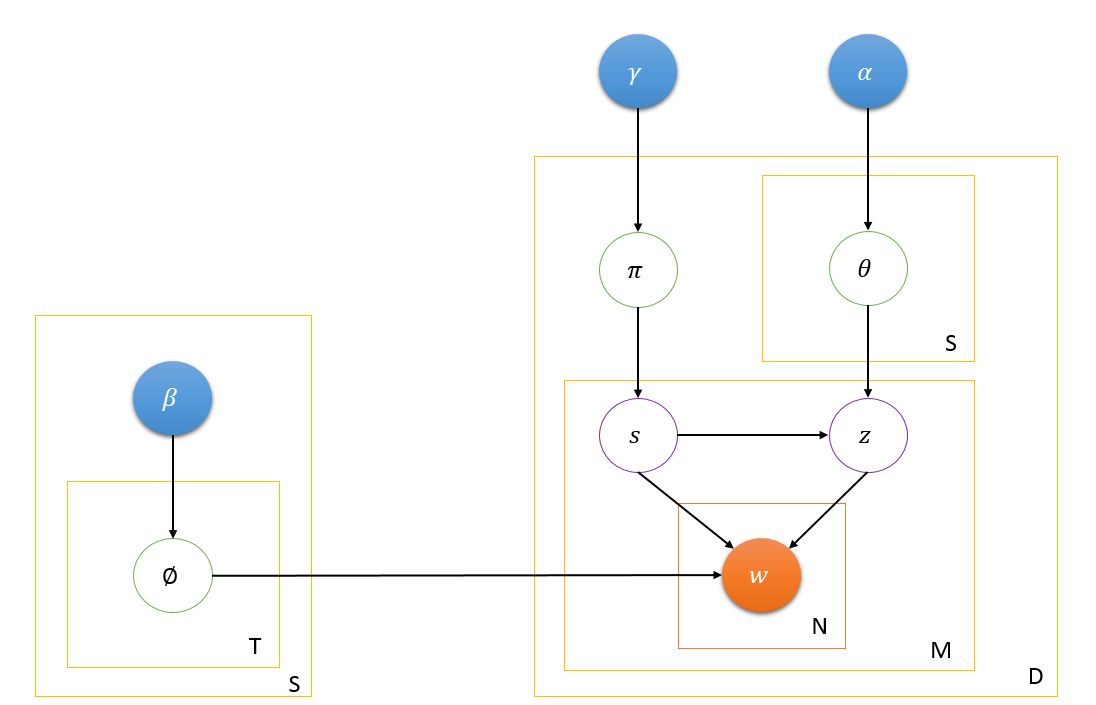
\includegraphics[width=\textwidth]{ASU}
   \caption{Aspect Sentiment Unification model}
   \label{asu}
\end{figure}


\section*{SUMMARY}
We introduced topic models with \textit{LDA} in section \ref{sec1}. The generative process and the inference method was explained in detail. The various applications
of topic models were discussed in section \ref{sec2}. Finally, in section \ref{sec3} we had a look at the generative models which combine topics and sentiment.

\bibliographystyle{abbrvnat}
\bibliography{Bibliography}

\end{document}
